% IEEE Paper Template for US-LETTER Page Size (V1)
% Sample Conference Paper using IEEE LaTeX style file for US-LETTER pagesize.
% Copyright (C) 2006-2008 Causal Productions Pty Ltd.
% Permission is granted to distribute and revise this file provided that
% this header remains intact.
%
% REVISION HISTORY
% 20080211 changed some space characters in the title-author block
%
\documentclass[10pt,conference,letterpaper]{IEEEtran}
\usepackage{times,amsmath,epsfig}

\usepackage{graphicx}
\usepackage{algorithm} % for algorithms
\usepackage{algpseudocode}
\algnewcommand{\LineComment}[1]{\State \(\triangleright\) #1} % for comments in line

\usepackage{booktabs} % For formal tables
%\usepackage{amsthm} % For claims  ???????

%
\title{Streaming text data classification}
%
\author{%
% author names are typeset in 11pt, which is the default size in the author block
{Igor E. Kuralenok{\small $~^{\#1}$}, 
    Nikita Marshalkin{\small $~^{\#2}$},
    Artem Trofimov{\small $~^{\#3}$}, 
    Boris Novikov{\small $~^{\#4}$},
    Mikhail Shavkunov{\small $~^{\#5}$}}%
% add some space between author names and affils
\vspace{1.6mm}\\
\fontsize{10}{10}\selectfont\itshape
% 20080211 CAUSAL PRODUCTIONS
% separate superscript on following line from affiliation using narrow space
$^{\#}$\,JetBrains Research\\
Saint Petersburg, Russia\\
\fontsize{9}{9}\selectfont\ttfamily\upshape
%
% 20080211 CAUSAL PRODUCTIONS
% in the following email addresses, separate the superscript from the email address 
% using a narrow space \,
% the reason is that Acrobat Reader has an option to auto-detect urls and email
% addresses, and make them 'hot'.  Without a narrow space, the superscript is included
% in the email address and corrupts it.
% Also, removed ~ from pre-superscript since it does not seem to serve any purpose
$^1$\,ikuralenok@gmail.com   %  \\
$^2$\,marnikitta@gmail.com    %  \\
$^3$\,trofimov9artem@gmail.com   % \\
$^4$\,borisnov@acm.org % \\
$^5$\,ololo@acm.org
}
%
\newcommand{\PicScale}{0.5}
\newcommand {\FlameStream} {FlameStream}

\begin{document}
\maketitle
%
\begin{abstract} 

\end{abstract}

% NOTE keywords are not used for conference papers so do not populate them
% \begin{keywords}
% keyword-1, keyword-2, keyword-3
% \end{keywords}
%
\section {Introduction}
%%% fs-seim-intro - Introduction

\label {fs-intro}

Nowadays, a lot of real-life applications use stream processing for network monitoring, financial analysis, training machine learning models, etc. State-of-the-art industrial stream processing systems, such as Flink \cite{carbone2015apache}, Samza \cite{Noghabi:2017:SSS:3137765.3137770}, Storm \cite{apache:storm}, Heron \cite{Kulkarni:2015:THS:2723372.2742788}, are able to provide low-latency and high-throughput in distributed environment for a wide range of analytical problems. However, issues related to the order-sensitive computations still remain. Most of these systems assume that events are fed to the system with monotonically increasing timestamps or with minor inversions. Often, such timestamps can be assigned at system's entry. Nevertheless, even if input items arrive at system's entry monotonically, they can be reordered because of parallel and asynchronous processing. In this case, order-sensitive operations located in data flow pipeline quite deeply can be broken. Figure ~\ref{break-order-dataflow} shows the example of common distributed stream processing pipeline that breaks the input order of operation, even if input events are monotonic and links between operations guarantee FIFO order. Basically, ordering constraints make sense only for stateful operations.

\begin{figure}[htbp]
  \centering
  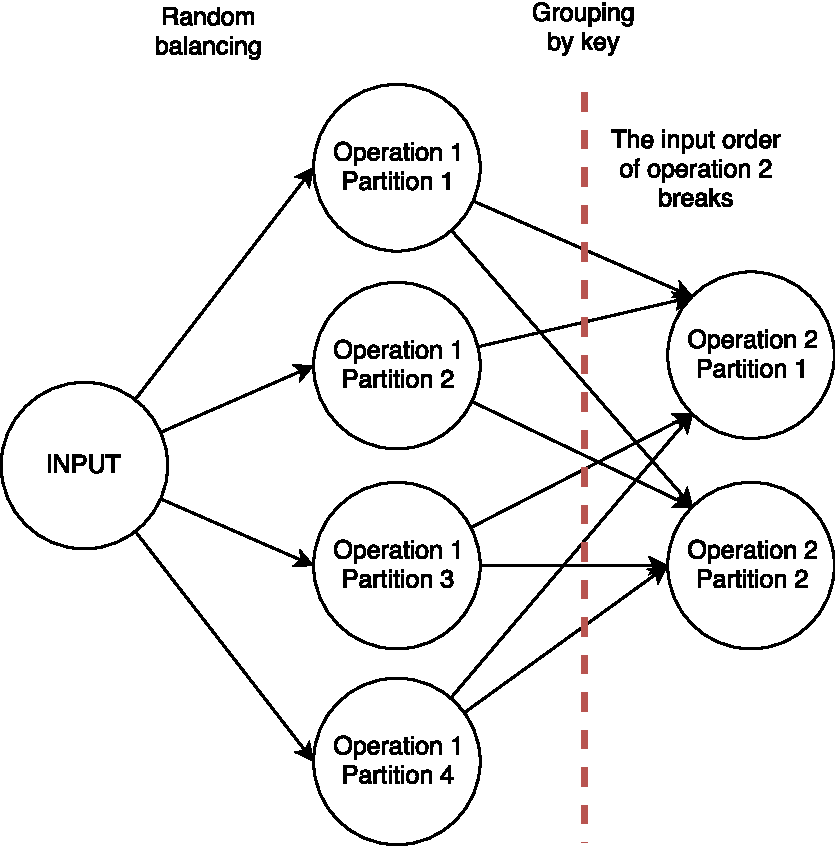
\includegraphics[width=0.38\textwidth]{pics/break_order_pipeline}
  \caption{An  example of common distributed stream processing pipeline that breaks the input order of operation}
  \label {break-order-dataflow}
\end{figure}

The typical way to achieve in-order processing is to buffer operation's input for some time to ensure that there are no out-of-order items. Most of the modern stream processing systems provide functionality to buffer all input items before specified operations until some user-provided conditions are satisfied. Conditions can be set on timing or the count of elements in the buffer. The main disadvantage of such techniques is that it can lead to significantly large latency, especially if the processing pipeline contains several operations that require ordered input. 

An alternative option is to handle out-of-order items as a special case in the business logic of operation. However, this way is suitable only for the limited number of tasks. Moreover, it may dramatically complicate the business-logic, which can lead to increasing the cost of its maintenance and is error-prone.
% sophisticated bugs.    

In this paper we propose an optimistic approach to handle out-of-order events in any stateful operation. In addition, we demonstrate its advantages compared to existing solutions. The contributions of this paper are the following: 

\begin {itemize}
\item Definition of new optimistic technique to handle out-of-order items in stateful operations
\item Demonstration of properties of this approach
\item Demonstration of working example that applies proposed method
\end {itemize}

The rest of the paper is structured as follows: in section~\ref{fs-stream} we formalize the preliminaries of stream processing, the examples of tasks that require ordered input are described in section~\ref{fs-tasks}, the typical approaches for handling out-of-order events are discussed in~\ref{fs-typical}, our optimistic technique is detailed in~\ref{fs-optimistic} and its performance is demonstrated in ~\ref{fs-experiments}, the main differences between proposed method and existing ones are shown in~\ref{fs-related}, finally we discuss the results and our plans in~\ref{fs-conclusion}.


\section{Experiments}
%%% fs-seim-experiments - Experiments

\label {fs-experiments}

In order to estimate the performance, we implemented a prototype based on the proposed approach. As a stream processing task, we apply the computation of inverted index for 1000 Wikipedia documents. The logical pipeline of this computation is shown in Figure ~\ref{inverted-index}. First map operation accepts Wikipedia documents and outputs pairs of words and corresponding positions. The next part of the pipeline accepts pairs of word and positions and computes updated posting list and the actual changelog. 

This stateful transformation is implemented in the form of groping and map operation with a cycle, as it was shown in the previous section. Regarding the physical deployment, the full logical graph is deployed on each computational unit or worker. Documents are randomly shuffled before the first map operation. Word positions are partitioned by word before grouping. The other links are implemented as simple chain calls.

\begin{figure}[htbp]
  \centering
  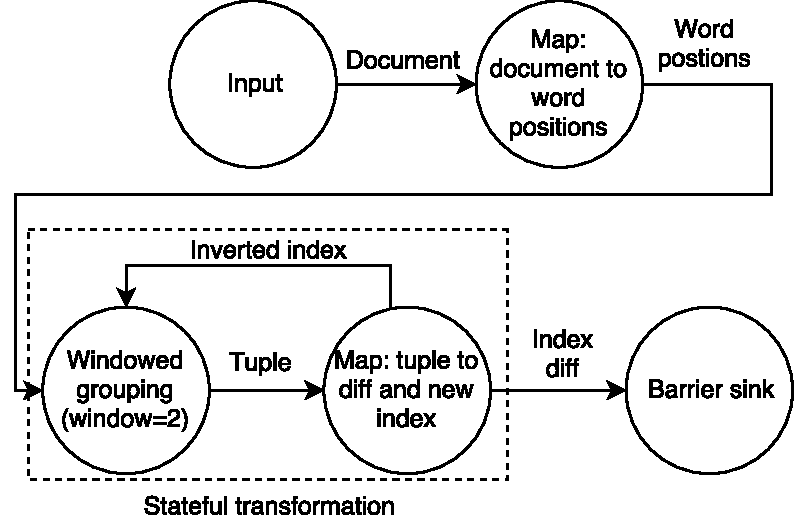
\includegraphics[width=0.48\textwidth]{pics/inverted-index}
  \caption{Logical pipeline for inverted index}
  \label {inverted-index}
\end{figure}

Our experiments were performed on clusters of 2, 4, 6, 8, and 10 nodes. Each node is an AWS EC2 micro instance with 1GB RAM and 1 core CPU.

As a key metric in our experiment, we take the ratio of arrived at the barrier items count to the number of the valid items among them. This value clearly represents the overhead of our approach, as it was mentioned at the end of the previous section. 

The relation between the number of workers, the delay between input documents and the proposed ratio is shown in Figure ~\ref{experiment}. As expected, the peak of the ratio is achieved when the document per second rate is high and the number of the nodes is low. This behaviour can be explained by the fact that a few workers cannot effectively deal with such intensive load. Nevertheless, the proportion of invalid items reduces with the increase of workers number. Under non-extreme load, the total overhead of the optimistic approach is under 10\% for all considered number of workers. These results confirm that the ratio does not increase with the growth of the number of nodes.

Therefore, the most important conclusions of the experiments are: the proposed method is scalable, the overhead could be optimized by system setup.

%% TODO: 
\begin{figure}[htbp]
  \centering
  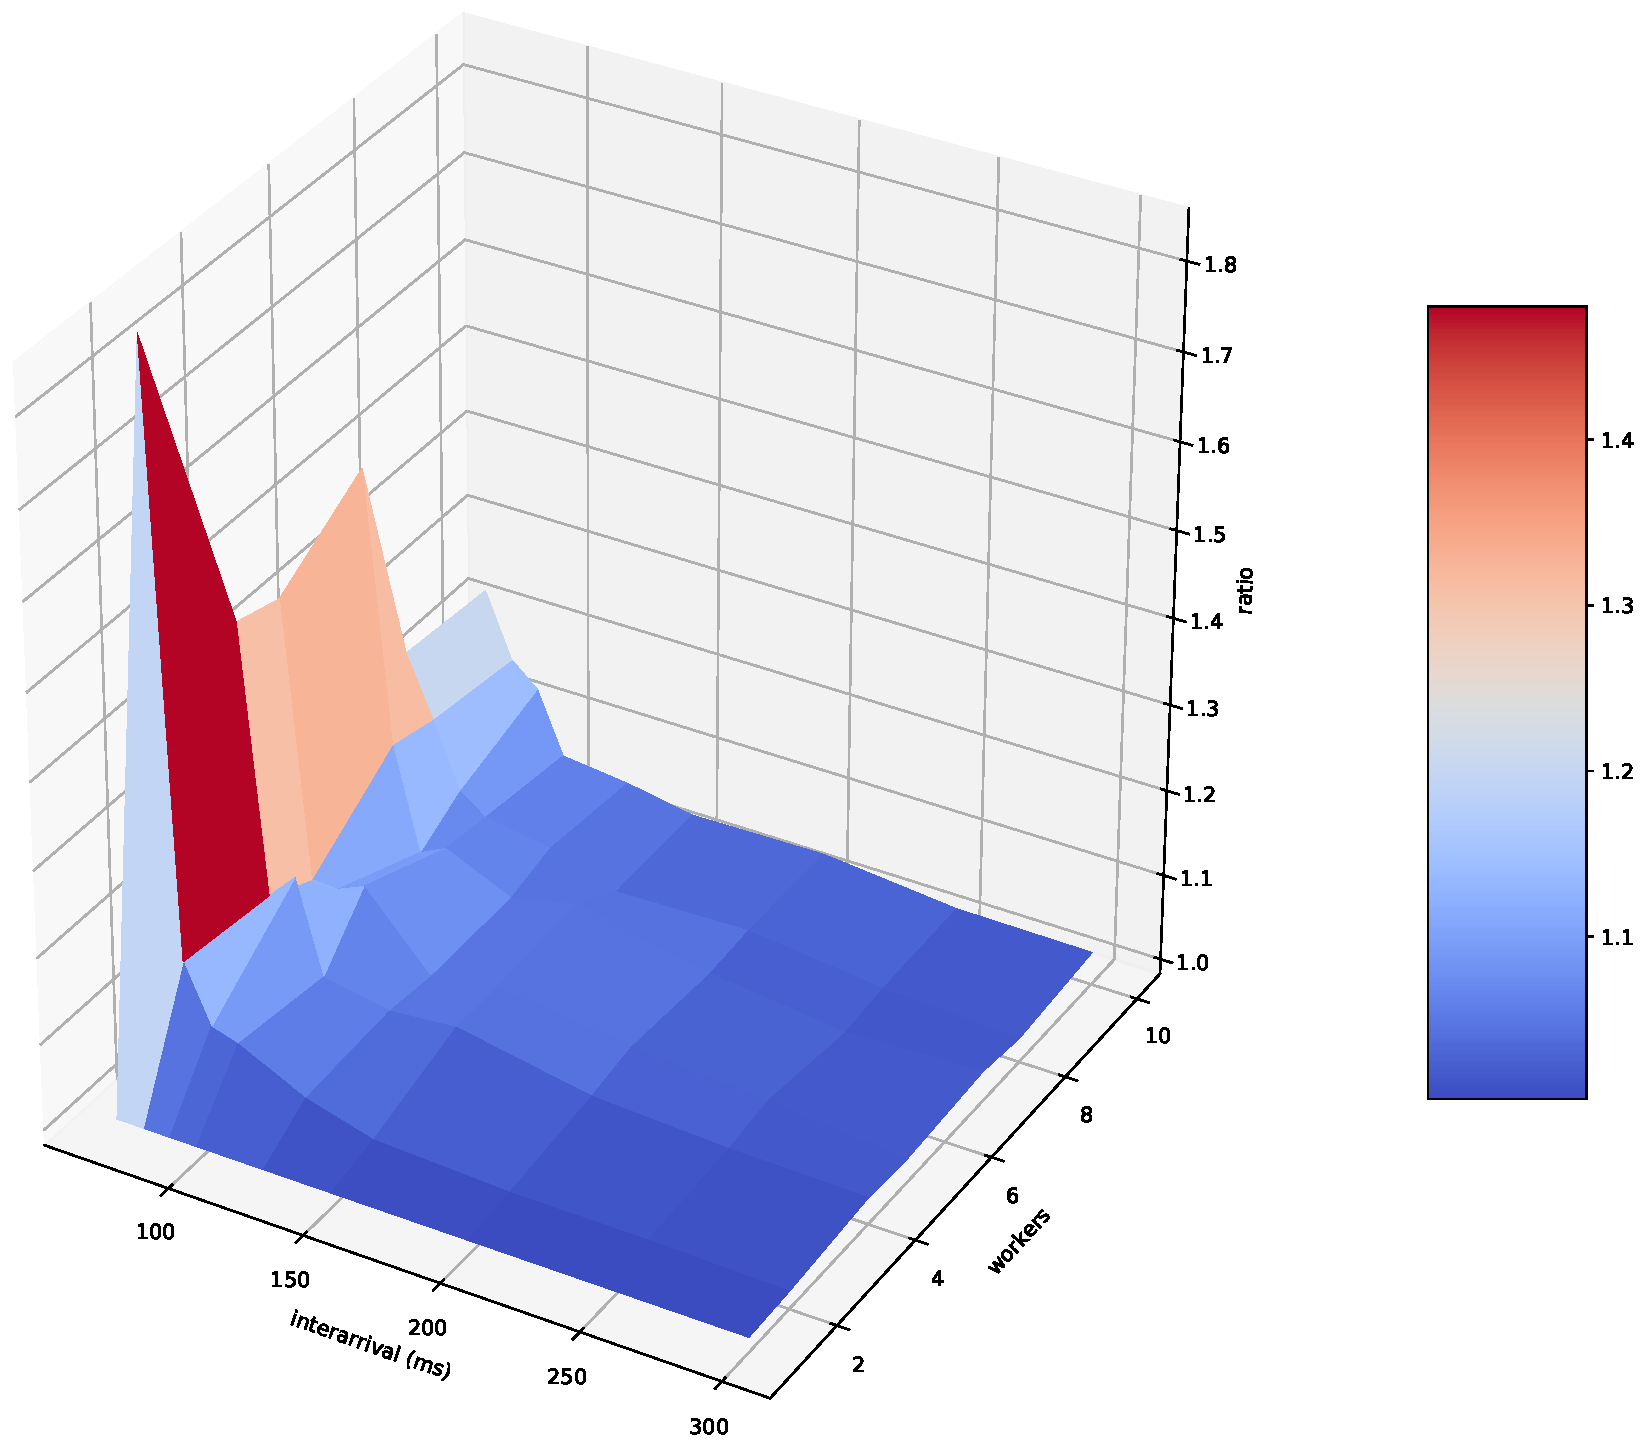
\includegraphics[width=0.48\textwidth]{pics/experiment}
  \caption{Experiment results}
  \label {experiment}
\end{figure}


\section{Related work}
%%% fs-seim-related - Related work

Seems to be related: \cite{4279071}, \cite{Wei:2009:SSO:1559845.1559973}, \cite{Mutschler:2014:ASP:2659232.2633686}.


\section{Conslusion}
%%% fs-seim-conclusion - Conclusion

\label {fs-conclusion}

In this paper we introduce an optimistic approach for handling out-of-order events. Our technique has the following key properties:

\begin{itemize}
    \item It does not require buffering before each order-sensitive operation
    \item The method handles properly any statful operation
    \item The overhead of the proposed approach is low and was under 10\% in most of our experiments
    \item The total overhead could be managed by optimization of the computational layout
\end{itemize}

The optimistic nature of this method is able to help to reduce the cost of waiting for punctuations or watermarks. It is implied by the fact, that at the moment when the watermark arrives all computations are already done. 

The experiments show that the number of the extra items does not increase with the growth of the number of the computational units. Therefore, this approach can potentially provide lower latency in stream processing systems.


\bibliographystyle{IEEEtran}
\bibliography{../../bibliography/flame-stream}

\end{document}

\endinput
